\documentclass[1p]{elsarticle_modified}
%\bibliographystyle{elsarticle-num}

%\usepackage[colorlinks]{hyperref}
%\usepackage{abbrmath_seonhwa} %\Abb, \Ascr, \Acal ,\Abf, \Afrak
\usepackage{amsfonts}
\usepackage{amssymb}
\usepackage{amsmath}
\usepackage{amsthm}
\usepackage{scalefnt}
\usepackage{amsbsy}
\usepackage{kotex}
\usepackage{caption}
\usepackage{subfig}
\usepackage{color}
\usepackage{graphicx}
\usepackage{xcolor} %% white, black, red, green, blue, cyan, magenta, yellow
\usepackage{float}
\usepackage{setspace}
\usepackage{hyperref}

\usepackage{tikz}
\usetikzlibrary{arrows}

\usepackage{multirow}
\usepackage{array} % fixed length table
\usepackage{hhline}

%%%%%%%%%%%%%%%%%%%%%
\makeatletter
\renewcommand*\env@matrix[1][\arraystretch]{%
	\edef\arraystretch{#1}%
	\hskip -\arraycolsep
	\let\@ifnextchar\new@ifnextchar
	\array{*\c@MaxMatrixCols c}}
\makeatother %https://tex.stackexchange.com/questions/14071/how-can-i-increase-the-line-spacing-in-a-matrix
%%%%%%%%%%%%%%%

\usepackage[normalem]{ulem}

\newcommand{\msout}[1]{\ifmmode\text{\sout{\ensuremath{#1}}}\else\sout{#1}\fi}
%SOURCE: \msout is \stkout macro in https://tex.stackexchange.com/questions/20609/strikeout-in-math-mode

\newcommand{\cancel}[1]{
	\ifmmode
	{\color{red}\msout{#1}}
	\else
	{\color{red}\sout{#1}}
	\fi
}

\newcommand{\add}[1]{
	{\color{blue}\uwave{#1}}
}

\newcommand{\replace}[2]{
	\ifmmode
	{\color{red}\msout{#1}}{\color{blue}\uwave{#2}}
	\else
	{\color{red}\sout{#1}}{\color{blue}\uwave{#2}}
	\fi
}

\newcommand{\Sol}{\mathcal{S}} %segment
\newcommand{\D}{D} %diagram
\newcommand{\A}{\mathcal{A}} %arc


%%%%%%%%%%%%%%%%%%%%%%%%%%%%%5 test

\def\sl{\operatorname{\textup{SL}}(2,\Cbb)}
\def\psl{\operatorname{\textup{PSL}}(2,\Cbb)}
\def\quan{\mkern 1mu \triangleright \mkern 1mu}

\theoremstyle{definition}
\newtheorem{thm}{Theorem}[section]
\newtheorem{prop}[thm]{Proposition}
\newtheorem{lem}[thm]{Lemma}
\newtheorem{ques}[thm]{Question}
\newtheorem{cor}[thm]{Corollary}
\newtheorem{defn}[thm]{Definition}
\newtheorem{exam}[thm]{Example}
\newtheorem{rmk}[thm]{Remark}
\newtheorem{alg}[thm]{Algorithm}

\newcommand{\I}{\sqrt{-1}}
\begin{document}

%\begin{frontmatter}
%
%\title{Boundary parabolic representations of knots up to 8 crossings}
%
%%% Group authors per affiliation:
%\author{Yunhi Cho} 
%\address{Department of Mathematics, University of Seoul, Seoul, Korea}
%\ead{yhcho@uos.ac.kr}
%
%
%\author{Seonhwa Kim} %\fnref{s_kim}}
%\address{Center for Geometry and Physics, Institute for Basic Science, Pohang, 37673, Korea}
%\ead{ryeona17@ibs.re.kr}
%
%\author{Hyuk Kim}
%\address{Department of Mathematical Sciences, Seoul National University, Seoul 08826, Korea}
%\ead{hyukkim@snu.ac.kr}
%
%\author{Seokbeom Yoon}
%\address{Department of Mathematical Sciences, Seoul National University, Seoul, 08826,  Korea}
%\ead{sbyoon15@snu.ac.kr}
%
%\begin{abstract}
%We find all boundary parabolic representation of knots up to 8 crossings.
%
%\end{abstract}
%\begin{keyword}
%    \MSC[2010] 57M25 
%\end{keyword}
%
%\end{frontmatter}

%\linenumbers
%\tableofcontents
%
\newcommand\colored[1]{\textcolor{white}{\rule[-0.35ex]{0.8em}{1.4ex}}\kern-0.8em\color{red} #1}%
%\newcommand\colored[1]{\textcolor{white}{ #1}\kern-2.17ex	\textcolor{white}{ #1}\kern-1.81ex	\textcolor{white}{ #1}\kern-2.15ex\color{red}#1	}

{\Large $\underline{11a_{320}~(K11a_{320})}$}

\setlength{\tabcolsep}{10pt}
\renewcommand{\arraystretch}{1.6}
\vspace{1cm}\begin{tabular}{m{100pt}>{\centering\arraybackslash}m{274pt}}
\multirow{5}{120pt}{
	\centering
	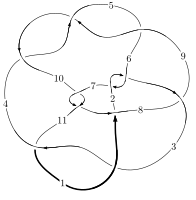
\includegraphics[width=112pt]{../../../GIT/diagram.site/Diagrams/png/569_11a_320.png}\\
\ \ \ A knot diagram\footnotemark}&
\allowdisplaybreaks
\textbf{Linearized knot diagam} \\
\cline{2-2}
 &
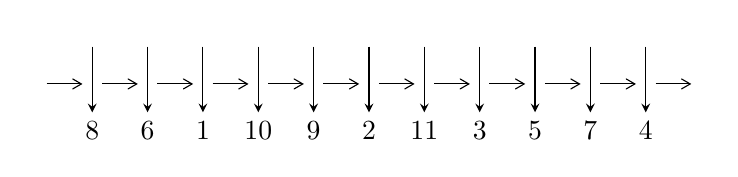
\begin{tikzpicture}[x=20pt, y=17pt]
	% nodes
	\node (C0) at (0, 0) {};
	\node (C1) at (1, 0) {};
	\node (C1U) at (1, +1) {};
	\node (C1D) at (1, -1) {8};

	\node (C2) at (2, 0) {};
	\node (C2U) at (2, +1) {};
	\node (C2D) at (2, -1) {6};

	\node (C3) at (3, 0) {};
	\node (C3U) at (3, +1) {};
	\node (C3D) at (3, -1) {1};

	\node (C4) at (4, 0) {};
	\node (C4U) at (4, +1) {};
	\node (C4D) at (4, -1) {10};

	\node (C5) at (5, 0) {};
	\node (C5U) at (5, +1) {};
	\node (C5D) at (5, -1) {9};

	\node (C6) at (6, 0) {};
	\node (C6U) at (6, +1) {};
	\node (C6D) at (6, -1) {2};

	\node (C7) at (7, 0) {};
	\node (C7U) at (7, +1) {};
	\node (C7D) at (7, -1) {11};

	\node (C8) at (8, 0) {};
	\node (C8U) at (8, +1) {};
	\node (C8D) at (8, -1) {3};

	\node (C9) at (9, 0) {};
	\node (C9U) at (9, +1) {};
	\node (C9D) at (9, -1) {5};

	\node (C10) at (10, 0) {};
	\node (C10U) at (10, +1) {};
	\node (C10D) at (10, -1) {7};

	\node (C11) at (11, 0) {};
	\node (C11U) at (11, +1) {};
	\node (C11D) at (11, -1) {4};
	\node (C12) at (12, 0) {};

	% arrows
	\draw[->,>={angle 60}]
	(C0) edge (C1) (C1) edge (C2) (C2) edge (C3) (C3) edge (C4) (C4) edge (C5) (C5) edge (C6) (C6) edge (C7) (C7) edge (C8) (C8) edge (C9) (C9) edge (C10) (C10) edge (C11) (C11) edge (C12) ;	\draw[->,>=stealth]
	(C1U) edge (C1D) (C2U) edge (C2D) (C3U) edge (C3D) (C4U) edge (C4D) (C5U) edge (C5D) (C6U) edge (C6D) (C7U) edge (C7D) (C8U) edge (C8D) (C9U) edge (C9D) (C10U) edge (C10D) (C11U) edge (C11D) ;
	\end{tikzpicture} \\
\hhline{~~} \\& 
\textbf{Solving Sequence} \\ \cline{2-2} 
 &
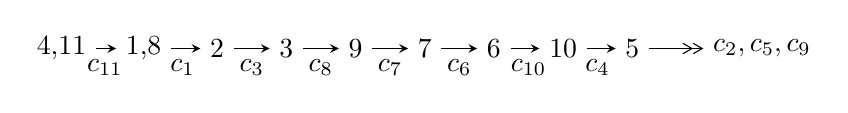
\begin{tikzpicture}[x=25pt, y=7pt]
	% node
	\node (A0) at (-1/8, 0) {4,11};
	\node (A1) at (17/16, 0) {1,8};
	\node (A2) at (17/8, 0) {2};
	\node (A3) at (25/8, 0) {3};
	\node (A4) at (33/8, 0) {9};
	\node (A5) at (41/8, 0) {7};
	\node (A6) at (49/8, 0) {6};
	\node (A7) at (57/8, 0) {10};
	\node (A8) at (65/8, 0) {5};
	\node (C1) at (1/2, -1) {$c_{11}$};
	\node (C2) at (13/8, -1) {$c_{1}$};
	\node (C3) at (21/8, -1) {$c_{3}$};
	\node (C4) at (29/8, -1) {$c_{8}$};
	\node (C5) at (37/8, -1) {$c_{7}$};
	\node (C6) at (45/8, -1) {$c_{6}$};
	\node (C7) at (53/8, -1) {$c_{10}$};
	\node (C8) at (61/8, -1) {$c_{4}$};
	\node (A9) at (10, 0) {$c_{2},c_{5},c_{9}$};

	% edge
	\draw[->,>=stealth]	
	(A0) edge (A1) (A1) edge (A2) (A2) edge (A3) (A3) edge (A4) (A4) edge (A5) (A5) edge (A6) (A6) edge (A7) (A7) edge (A8) ;
	\draw[->>,>={angle 60}]	
	(A8) edge (A9);
\end{tikzpicture} \\ 

\end{tabular} \\

\footnotetext{
The image of knot diagram is generated by the software ``\textbf{Draw programme}" developed by Andrew Bartholomew(\url{http://www.layer8.co.uk/maths/draw/index.htm\#Running-draw}), where we modified some parts for our purpose(\url{https://github.com/CATsTAILs/LinksPainter}).
}\phantom \\ \newline 
\centering \textbf{Ideals for irreducible components\footnotemark of $X_{\text{par}}$} 
 
\begin{align*}
I^u_{1}&=\langle 
-5.12599\times10^{149} u^{70}+2.15209\times10^{150} u^{69}+\cdots+5.93070\times10^{149} b+5.39933\times10^{150},\\
\phantom{I^u_{1}}&\phantom{= \langle  }8.74134\times10^{150} u^{70}-2.86993\times10^{151} u^{69}+\cdots+1.12683\times10^{151} a+2.95601\times10^{152},\\
\phantom{I^u_{1}}&\phantom{= \langle  }u^{71}-4 u^{70}+\cdots-82 u+19\rangle \\
I^u_{2}&=\langle 
-4 u^{16}+17 u^{15}+\cdots+b-13,\;2 u^{16}-9 u^{15}+\cdots+a+9,\;u^{17}-3 u^{16}+\cdots+3 u-1\rangle \\
\\
\end{align*}
\raggedright * 2 irreducible components of $\dim_{\mathbb{C}}=0$, with total 88 representations.\\
\footnotetext{All coefficients of polynomials are rational numbers. But the coefficients are sometimes approximated in decimal forms when there is not enough margin.}
\newpage
\renewcommand{\arraystretch}{1}
\centering \section*{I. $I^u_{1}= \langle -5.13\times10^{149} u^{70}+2.15\times10^{150} u^{69}+\cdots+5.93\times10^{149} b+5.40\times10^{150},\;8.74\times10^{150} u^{70}-2.87\times10^{151} u^{69}+\cdots+1.13\times10^{151} a+2.96\times10^{152},\;u^{71}-4 u^{70}+\cdots-82 u+19 \rangle$}
\flushleft \textbf{(i) Arc colorings}\\
\begin{tabular}{m{7pt} m{180pt} m{7pt} m{180pt} }
\flushright $a_{4}=$&$\begin{pmatrix}0\\u\end{pmatrix}$ \\
\flushright $a_{11}=$&$\begin{pmatrix}1\\0\end{pmatrix}$ \\
\flushright $a_{1}=$&$\begin{pmatrix}1\\u^2\end{pmatrix}$ \\
\flushright $a_{8}=$&$\begin{pmatrix}-0.775744 u^{70}+2.54690 u^{69}+\cdots+40.6903 u-26.2329\\0.864314 u^{70}-3.62872 u^{69}+\cdots+57.6823 u-9.10403\end{pmatrix}$ \\
\flushright $a_{2}=$&$\begin{pmatrix}0.181619 u^{70}-0.0673367 u^{69}+\cdots-185.458 u+42.0713\\0.130604 u^{70}-0.388077 u^{69}+\cdots-12.6153 u-0.350324\end{pmatrix}$ \\
\flushright $a_{3}=$&$\begin{pmatrix}u\\u^3+u\end{pmatrix}$ \\
\flushright $a_{9}=$&$\begin{pmatrix}0.0637919 u^{70}-0.858245 u^{69}+\cdots+60.8860 u-25.1281\\0.857701 u^{70}-3.68006 u^{69}+\cdots+58.0726 u-7.10612\end{pmatrix}$ \\
\flushright $a_{7}=$&$\begin{pmatrix}0.0885694 u^{70}-1.08182 u^{69}+\cdots+98.3726 u-35.3370\\0.864314 u^{70}-3.62872 u^{69}+\cdots+57.6823 u-9.10403\end{pmatrix}$ \\
\flushright $a_{6}=$&$\begin{pmatrix}0.680313 u^{70}-1.71230 u^{69}+\cdots-22.8206 u+17.1395\\0.0264002 u^{70}+0.0383447 u^{69}+\cdots-35.8478 u+8.50989\end{pmatrix}$ \\
\flushright $a_{10}=$&$\begin{pmatrix}-0.0235381 u^{70}+0.0777773 u^{69}+\cdots+12.0205 u+5.65632\\-0.396807 u^{70}+2.02745 u^{69}+\cdots-31.9176 u+9.02563\end{pmatrix}$ \\
\flushright $a_{5}=$&$\begin{pmatrix}-0.521650 u^{70}+3.14454 u^{69}+\cdots-204.598 u+45.3905\\0.309001 u^{70}-0.338161 u^{69}+\cdots-72.8831 u+18.8315\end{pmatrix}$\\ \flushright $a_{5}=$&$\begin{pmatrix}-0.521650 u^{70}+3.14454 u^{69}+\cdots-204.598 u+45.3905\\0.309001 u^{70}-0.338161 u^{69}+\cdots-72.8831 u+18.8315\end{pmatrix}$\\&\end{tabular}
\flushleft \textbf{(ii) Obstruction class $= -1$}\\~\\
\flushleft \textbf{(iii) Cusp Shapes $= 1.74408 u^{70}-7.67739 u^{69}+\cdots+186.830 u-24.0299$}\\~\\
\newpage\renewcommand{\arraystretch}{1}
\flushleft \textbf{(iv) u-Polynomials at the component}\newline \\
\begin{tabular}{m{50pt}|m{274pt}}
Crossings & \hspace{64pt}u-Polynomials at each crossing \\
\hline $$\begin{aligned}c_{1}\end{aligned}$$&$\begin{aligned}
&u^{71}- u^{70}+\cdots-253 u+121
\end{aligned}$\\
\hline $$\begin{aligned}c_{2},c_{6}\end{aligned}$$&$\begin{aligned}
&u^{71}+2 u^{70}+\cdots+212 u+103
\end{aligned}$\\
\hline $$\begin{aligned}c_{3},c_{11}\end{aligned}$$&$\begin{aligned}
&u^{71}-4 u^{70}+\cdots-82 u+19
\end{aligned}$\\
\hline $$\begin{aligned}c_{4},c_{5},c_{9}\end{aligned}$$&$\begin{aligned}
&u^{71}+u^{70}+\cdots-9 u+11
\end{aligned}$\\
\hline $$\begin{aligned}c_{7},c_{10}\end{aligned}$$&$\begin{aligned}
&u^{71}-18 u^{69}+\cdots+28 u+19
\end{aligned}$\\
\hline $$\begin{aligned}c_{8}\end{aligned}$$&$\begin{aligned}
&u^{71}+u^{70}+\cdots+75261 u+69721
\end{aligned}$\\
\hline
\end{tabular}\\~\\
\newpage\renewcommand{\arraystretch}{1}
\flushleft \textbf{(v) Riley Polynomials at the component}\newline \\
\begin{tabular}{m{50pt}|m{274pt}}
Crossings & \hspace{64pt}Riley Polynomials at each crossing \\
\hline $$\begin{aligned}c_{1}\end{aligned}$$&$\begin{aligned}
&y^{71}+13 y^{70}+\cdots-110473 y-14641
\end{aligned}$\\
\hline $$\begin{aligned}c_{2},c_{6}\end{aligned}$$&$\begin{aligned}
&y^{71}+52 y^{70}+\cdots-123976 y-10609
\end{aligned}$\\
\hline $$\begin{aligned}c_{3},c_{11}\end{aligned}$$&$\begin{aligned}
&y^{71}+48 y^{70}+\cdots-4562 y-361
\end{aligned}$\\
\hline $$\begin{aligned}c_{4},c_{5},c_{9}\end{aligned}$$&$\begin{aligned}
&y^{71}+77 y^{70}+\cdots+103 y-121
\end{aligned}$\\
\hline $$\begin{aligned}c_{7},c_{10}\end{aligned}$$&$\begin{aligned}
&y^{71}-36 y^{70}+\cdots+9258 y-361
\end{aligned}$\\
\hline $$\begin{aligned}c_{8}\end{aligned}$$&$\begin{aligned}
&y^{71}+37 y^{70}+\cdots-78658032583 y-4861017841
\end{aligned}$\\
\hline
\end{tabular}\\~\\
\newpage\flushleft \textbf{(vi) Complex Volumes and Cusp Shapes}
$$\begin{array}{c|c|c}  
\text{Solutions to }I^u_{1}& \I (\text{vol} + \sqrt{-1}CS) & \text{Cusp shape}\\
 \hline 
\begin{aligned}
u &= \phantom{-}0.047825 + 1.017730 I \\
a &= -0.341643 - 0.579404 I \\
b &= \phantom{-}1.69982 + 0.31305 I\end{aligned}
 & \phantom{-}3.38826 - 2.90800 I & \phantom{-0.000000 } 0 \\ \hline\begin{aligned}
u &= \phantom{-}0.047825 - 1.017730 I \\
a &= -0.341643 + 0.579404 I \\
b &= \phantom{-}1.69982 - 0.31305 I\end{aligned}
 & \phantom{-}3.38826 + 2.90800 I & \phantom{-0.000000 } 0 \\ \hline\begin{aligned}
u &= \phantom{-}0.423933 + 0.883947 I \\
a &= -0.940566 - 0.386865 I \\
b &= \phantom{-}1.128290 - 0.272503 I\end{aligned}
 & \phantom{-}3.17690 + 1.80430 I & \phantom{-0.000000 } 0 \\ \hline\begin{aligned}
u &= \phantom{-}0.423933 - 0.883947 I \\
a &= -0.940566 + 0.386865 I \\
b &= \phantom{-}1.128290 + 0.272503 I\end{aligned}
 & \phantom{-}3.17690 - 1.80430 I & \phantom{-0.000000 } 0 \\ \hline\begin{aligned}
u &= \phantom{-}0.336740 + 0.978403 I \\
a &= \phantom{-}0.11372 - 1.77123 I \\
b &= \phantom{-}1.15954 + 0.90500 I\end{aligned}
 & \phantom{-}3.89503 - 4.72871 I & \phantom{-0.000000 } 0 \\ \hline\begin{aligned}
u &= \phantom{-}0.336740 - 0.978403 I \\
a &= \phantom{-}0.11372 + 1.77123 I \\
b &= \phantom{-}1.15954 - 0.90500 I\end{aligned}
 & \phantom{-}3.89503 + 4.72871 I & \phantom{-0.000000 } 0 \\ \hline\begin{aligned}
u &= -0.754094 + 0.580048 I \\
a &= -0.547122 - 0.007044 I \\
b &= \phantom{-}1.096540 + 0.755338 I\end{aligned}
 & \phantom{-}4.98219 - 1.09775 I & \phantom{-0.000000 } 0 \\ \hline\begin{aligned}
u &= -0.754094 - 0.580048 I \\
a &= -0.547122 + 0.007044 I \\
b &= \phantom{-}1.096540 - 0.755338 I\end{aligned}
 & \phantom{-}4.98219 + 1.09775 I & \phantom{-0.000000 } 0 \\ \hline\begin{aligned}
u &= \phantom{-}0.046777 + 1.050160 I \\
a &= \phantom{-}0.09283 - 2.20296 I \\
b &= -0.706702 + 0.426522 I\end{aligned}
 & \phantom{-}4.71218 - 0.33668 I & \phantom{-0.000000 } 0 \\ \hline\begin{aligned}
u &= \phantom{-}0.046777 - 1.050160 I \\
a &= \phantom{-}0.09283 + 2.20296 I \\
b &= -0.706702 - 0.426522 I\end{aligned}
 & \phantom{-}4.71218 + 0.33668 I & \phantom{-0.000000 } 0\\
 \hline 
 \end{array}$$\newpage$$\begin{array}{c|c|c}  
\text{Solutions to }I^u_{1}& \I (\text{vol} + \sqrt{-1}CS) & \text{Cusp shape}\\
 \hline 
\begin{aligned}
u &= \phantom{-}0.942608 + 0.017959 I \\
a &= \phantom{-}0.343675 + 0.335171 I \\
b &= \phantom{-}1.144670 - 0.403404 I\end{aligned}
 & -0.32112 + 5.84881 I & \phantom{-0.000000 } 0 \\ \hline\begin{aligned}
u &= \phantom{-}0.942608 - 0.017959 I \\
a &= \phantom{-}0.343675 - 0.335171 I \\
b &= \phantom{-}1.144670 + 0.403404 I\end{aligned}
 & -0.32112 - 5.84881 I & \phantom{-0.000000 } 0 \\ \hline\begin{aligned}
u &= -0.232384 + 1.034920 I \\
a &= -0.173815 - 0.997337 I \\
b &= \phantom{-}0.299021 + 0.503997 I\end{aligned}
 & \phantom{-}2.02658 + 2.02846 I & \phantom{-0.000000 } 0 \\ \hline\begin{aligned}
u &= -0.232384 - 1.034920 I \\
a &= -0.173815 + 0.997337 I \\
b &= \phantom{-}0.299021 - 0.503997 I\end{aligned}
 & \phantom{-}2.02658 - 2.02846 I & \phantom{-0.000000 } 0 \\ \hline\begin{aligned}
u &= \phantom{-}0.200339 + 0.907089 I \\
a &= \phantom{-}0.25180 + 1.54170 I \\
b &= -0.999500 - 0.475840 I\end{aligned}
 & -0.352598 - 1.166030 I & \phantom{-0.000000 } 0 \\ \hline\begin{aligned}
u &= \phantom{-}0.200339 - 0.907089 I \\
a &= \phantom{-}0.25180 - 1.54170 I \\
b &= -0.999500 + 0.475840 I\end{aligned}
 & -0.352598 + 1.166030 I & \phantom{-0.000000 } 0 \\ \hline\begin{aligned}
u &= \phantom{-}0.842416 + 0.377347 I \\
a &= -1.129690 + 0.265067 I \\
b &= -0.468514 + 0.604687 I\end{aligned}
 & \phantom{-}8.76103 - 4.23637 I & \phantom{-0.000000 } 0 \\ \hline\begin{aligned}
u &= \phantom{-}0.842416 - 0.377347 I \\
a &= -1.129690 - 0.265067 I \\
b &= -0.468514 - 0.604687 I\end{aligned}
 & \phantom{-}8.76103 + 4.23637 I & \phantom{-0.000000 } 0 \\ \hline\begin{aligned}
u &= -0.353533 + 1.029640 I \\
a &= \phantom{-}0.41833 - 1.67791 I \\
b &= -0.972971 + 0.871224 I\end{aligned}
 & \phantom{-}0.74759 + 4.36932 I & \phantom{-0.000000 } 0 \\ \hline\begin{aligned}
u &= -0.353533 - 1.029640 I \\
a &= \phantom{-}0.41833 + 1.67791 I \\
b &= -0.972971 - 0.871224 I\end{aligned}
 & \phantom{-}0.74759 - 4.36932 I & \phantom{-0.000000 } 0\\
 \hline 
 \end{array}$$\newpage$$\begin{array}{c|c|c}  
\text{Solutions to }I^u_{1}& \I (\text{vol} + \sqrt{-1}CS) & \text{Cusp shape}\\
 \hline 
\begin{aligned}
u &= -0.569298 + 0.933529 I \\
a &= \phantom{-}0.28166 + 1.90992 I \\
b &= \phantom{-}0.99993 - 1.09682 I\end{aligned}
 & \phantom{-}6.02225 + 6.08511 I & \phantom{-0.000000 } 0 \\ \hline\begin{aligned}
u &= -0.569298 - 0.933529 I \\
a &= \phantom{-}0.28166 - 1.90992 I \\
b &= \phantom{-}0.99993 + 1.09682 I\end{aligned}
 & \phantom{-}6.02225 - 6.08511 I & \phantom{-0.000000 } 0 \\ \hline\begin{aligned}
u &= \phantom{-}0.048283 + 1.137300 I \\
a &= -0.949590 + 0.745505 I \\
b &= \phantom{-}0.988491 - 0.625407 I\end{aligned}
 & \phantom{-}3.52458 + 2.13444 I & \phantom{-0.000000 } 0 \\ \hline\begin{aligned}
u &= \phantom{-}0.048283 - 1.137300 I \\
a &= -0.949590 - 0.745505 I \\
b &= \phantom{-}0.988491 + 0.625407 I\end{aligned}
 & \phantom{-}3.52458 - 2.13444 I & \phantom{-0.000000 } 0 \\ \hline\begin{aligned}
u &= -1.123150 + 0.278639 I \\
a &= \phantom{-}0.341249 - 0.025673 I \\
b &= \phantom{-}0.965387 + 0.144697 I\end{aligned}
 & -3.38978 - 0.40278 I & \phantom{-0.000000 } 0 \\ \hline\begin{aligned}
u &= -1.123150 - 0.278639 I \\
a &= \phantom{-}0.341249 + 0.025673 I \\
b &= \phantom{-}0.965387 - 0.144697 I\end{aligned}
 & -3.38978 + 0.40278 I & \phantom{-0.000000 } 0 \\ \hline\begin{aligned}
u &= -0.134492 + 1.169680 I \\
a &= \phantom{-}0.67489 + 1.48395 I \\
b &= \phantom{-}1.082810 - 0.501331 I\end{aligned}
 & \phantom{-}10.90650 + 5.21367 I & \phantom{-0.000000 } 0 \\ \hline\begin{aligned}
u &= -0.134492 - 1.169680 I \\
a &= \phantom{-}0.67489 - 1.48395 I \\
b &= \phantom{-}1.082810 + 0.501331 I\end{aligned}
 & \phantom{-}10.90650 - 5.21367 I & \phantom{-0.000000 } 0 \\ \hline\begin{aligned}
u &= \phantom{-}0.582442 + 1.060300 I \\
a &= \phantom{-}0.724590 - 1.097650 I \\
b &= \phantom{-}0.651275 + 0.464021 I\end{aligned}
 & \phantom{-}4.88583 - 2.21298 I & \phantom{-0.000000 } 0 \\ \hline\begin{aligned}
u &= \phantom{-}0.582442 - 1.060300 I \\
a &= \phantom{-}0.724590 + 1.097650 I \\
b &= \phantom{-}0.651275 - 0.464021 I\end{aligned}
 & \phantom{-}4.88583 + 2.21298 I & \phantom{-0.000000 } 0\\
 \hline 
 \end{array}$$\newpage$$\begin{array}{c|c|c}  
\text{Solutions to }I^u_{1}& \I (\text{vol} + \sqrt{-1}CS) & \text{Cusp shape}\\
 \hline 
\begin{aligned}
u &= \phantom{-}0.327594 + 1.168440 I \\
a &= -0.53229 + 1.43066 I \\
b &= \phantom{-}0.321204 - 1.006900 I\end{aligned}
 & \phantom{-}6.37762 - 5.16098 I & \phantom{-0.000000 } 0 \\ \hline\begin{aligned}
u &= \phantom{-}0.327594 - 1.168440 I \\
a &= -0.53229 - 1.43066 I \\
b &= \phantom{-}0.321204 + 1.006900 I\end{aligned}
 & \phantom{-}6.37762 + 5.16098 I & \phantom{-0.000000 } 0 \\ \hline\begin{aligned}
u &= -0.447415 + 1.183120 I \\
a &= \phantom{-}0.405310 - 1.254470 I \\
b &= -0.719914 + 0.311279 I\end{aligned}
 & \phantom{-}0.95702 + 2.39465 I & \phantom{-0.000000 } 0 \\ \hline\begin{aligned}
u &= -0.447415 - 1.183120 I \\
a &= \phantom{-}0.405310 + 1.254470 I \\
b &= -0.719914 - 0.311279 I\end{aligned}
 & \phantom{-}0.95702 - 2.39465 I & \phantom{-0.000000 } 0 \\ \hline\begin{aligned}
u &= \phantom{-}1.289830 + 0.094787 I \\
a &= -0.206069 - 0.147386 I \\
b &= -1.061290 + 0.595628 I\end{aligned}
 & \phantom{-}7.03255 + 9.09735 I & \phantom{-0.000000 } 0 \\ \hline\begin{aligned}
u &= \phantom{-}1.289830 - 0.094787 I \\
a &= -0.206069 + 0.147386 I \\
b &= -1.061290 - 0.595628 I\end{aligned}
 & \phantom{-}7.03255 - 9.09735 I & \phantom{-0.000000 } 0 \\ \hline\begin{aligned}
u &= -0.574723 + 0.330407 I \\
a &= -0.538480 + 0.587756 I \\
b &= -1.118760 + 0.110427 I\end{aligned}
 & -1.79167 + 1.75090 I & -12.48087 - 4.54784 I \\ \hline\begin{aligned}
u &= -0.574723 - 0.330407 I \\
a &= -0.538480 - 0.587756 I \\
b &= -1.118760 - 0.110427 I\end{aligned}
 & -1.79167 - 1.75090 I & -12.48087 + 4.54784 I \\ \hline\begin{aligned}
u &= \phantom{-}0.384607 + 1.314120 I \\
a &= \phantom{-}0.469556 - 1.191940 I \\
b &= -0.54031 + 1.32564 I\end{aligned}
 & \phantom{-}13.6021 - 8.3409 I & \phantom{-0.000000 } 0 \\ \hline\begin{aligned}
u &= \phantom{-}0.384607 - 1.314120 I \\
a &= \phantom{-}0.469556 + 1.191940 I \\
b &= -0.54031 - 1.32564 I\end{aligned}
 & \phantom{-}13.6021 + 8.3409 I & \phantom{-0.000000 } 0\\
 \hline 
 \end{array}$$\newpage$$\begin{array}{c|c|c}  
\text{Solutions to }I^u_{1}& \I (\text{vol} + \sqrt{-1}CS) & \text{Cusp shape}\\
 \hline 
\begin{aligned}
u &= \phantom{-}0.271650 + 1.343530 I \\
a &= \phantom{-}0.82251 + 1.49102 I \\
b &= -0.977413 - 0.493272 I\end{aligned}
 & \phantom{-}3.76513 - 4.21784 I & \phantom{-0.000000 } 0 \\ \hline\begin{aligned}
u &= \phantom{-}0.271650 - 1.343530 I \\
a &= \phantom{-}0.82251 - 1.49102 I \\
b &= -0.977413 + 0.493272 I\end{aligned}
 & \phantom{-}3.76513 + 4.21784 I & \phantom{-0.000000 } 0 \\ \hline\begin{aligned}
u &= -0.558176 + 1.269410 I \\
a &= -0.071999 + 1.263220 I \\
b &= \phantom{-}1.071650 - 0.517844 I\end{aligned}
 & -0.06369 + 6.26228 I & \phantom{-0.000000 } 0 \\ \hline\begin{aligned}
u &= -0.558176 - 1.269410 I \\
a &= -0.071999 - 1.263220 I \\
b &= \phantom{-}1.071650 + 0.517844 I\end{aligned}
 & -0.06369 - 6.26228 I & \phantom{-0.000000 } 0 \\ \hline\begin{aligned}
u &= \phantom{-}0.255272 + 0.548146 I \\
a &= -1.01679 - 1.14079 I \\
b &= \phantom{-}0.788104 - 0.383173 I\end{aligned}
 & \phantom{-}2.89013 + 1.78350 I & -4.97596 - 3.66282 I \\ \hline\begin{aligned}
u &= \phantom{-}0.255272 - 0.548146 I \\
a &= -1.01679 + 1.14079 I \\
b &= \phantom{-}0.788104 + 0.383173 I\end{aligned}
 & \phantom{-}2.89013 - 1.78350 I & -4.97596 + 3.66282 I \\ \hline\begin{aligned}
u &= \phantom{-}0.48232 + 1.33424 I \\
a &= -0.25643 - 1.55861 I \\
b &= \phantom{-}1.173600 + 0.644507 I\end{aligned}
 & \phantom{-}3.81421 - 11.00460 I & \phantom{-0.000000 } 0 \\ \hline\begin{aligned}
u &= \phantom{-}0.48232 - 1.33424 I \\
a &= -0.25643 + 1.55861 I \\
b &= \phantom{-}1.173600 - 0.644507 I\end{aligned}
 & \phantom{-}3.81421 + 11.00460 I & \phantom{-0.000000 } 0 \\ \hline\begin{aligned}
u &= -0.26701 + 1.39737 I \\
a &= \phantom{-}0.073429 + 1.010430 I \\
b &= -0.207375 - 1.100390 I\end{aligned}
 & \phantom{-}9.45981 + 2.99993 I & \phantom{-0.000000 } 0 \\ \hline\begin{aligned}
u &= -0.26701 - 1.39737 I \\
a &= \phantom{-}0.073429 - 1.010430 I \\
b &= -0.207375 + 1.100390 I\end{aligned}
 & \phantom{-}9.45981 - 2.99993 I & \phantom{-0.000000 } 0\\
 \hline 
 \end{array}$$\newpage$$\begin{array}{c|c|c}  
\text{Solutions to }I^u_{1}& \I (\text{vol} + \sqrt{-1}CS) & \text{Cusp shape}\\
 \hline 
\begin{aligned}
u &= \phantom{-}0.571182 + 0.076246 I \\
a &= \phantom{-}0.752333 + 0.565781 I \\
b &= \phantom{-}0.072263 - 0.698701 I\end{aligned}
 & \phantom{-}2.82580 - 1.80720 I & -7.38072 + 3.47906 I \\ \hline\begin{aligned}
u &= \phantom{-}0.571182 - 0.076246 I \\
a &= \phantom{-}0.752333 - 0.565781 I \\
b &= \phantom{-}0.072263 + 0.698701 I\end{aligned}
 & \phantom{-}2.82580 + 1.80720 I & -7.38072 - 3.47906 I \\ \hline\begin{aligned}
u &= -1.40638 + 0.36204 I \\
a &= -0.332339 - 0.060821 I \\
b &= -0.869643 - 0.457967 I\end{aligned}
 & \phantom{-}2.53123 - 1.88371 I & \phantom{-0.000000 } 0 \\ \hline\begin{aligned}
u &= -1.40638 - 0.36204 I \\
a &= -0.332339 + 0.060821 I \\
b &= -0.869643 + 0.457967 I\end{aligned}
 & \phantom{-}2.53123 + 1.88371 I & \phantom{-0.000000 } 0 \\ \hline\begin{aligned}
u &= \phantom{-}0.350880 + 0.384879 I \\
a &= \phantom{-}0.319220 + 1.255840 I \\
b &= -1.248260 - 0.193640 I\end{aligned}
 & -1.10877 - 1.58604 I & -13.47873 + 2.62387 I \\ \hline\begin{aligned}
u &= \phantom{-}0.350880 - 0.384879 I \\
a &= \phantom{-}0.319220 - 1.255840 I \\
b &= -1.248260 + 0.193640 I\end{aligned}
 & -1.10877 + 1.58604 I & -13.47873 - 2.62387 I \\ \hline\begin{aligned}
u &= \phantom{-}0.71970 + 1.29915 I \\
a &= -0.512729 + 0.883109 I \\
b &= -1.073070 - 0.541535 I\end{aligned}
 & \phantom{-}11.25790 - 1.96679 I & \phantom{-0.000000 } 0 \\ \hline\begin{aligned}
u &= \phantom{-}0.71970 - 1.29915 I \\
a &= -0.512729 - 0.883109 I \\
b &= -1.073070 + 0.541535 I\end{aligned}
 & \phantom{-}11.25790 + 1.96679 I & \phantom{-0.000000 } 0 \\ \hline\begin{aligned}
u &= \phantom{-}0.117612 + 0.490736 I \\
a &= -3.12111 + 2.61533 I \\
b &= \phantom{-}0.283166 + 0.342632 I\end{aligned}
 & \phantom{-}8.37213 - 4.43001 I & -3.16531 - 0.91454 I \\ \hline\begin{aligned}
u &= \phantom{-}0.117612 - 0.490736 I \\
a &= -3.12111 - 2.61533 I \\
b &= \phantom{-}0.283166 - 0.342632 I\end{aligned}
 & \phantom{-}8.37213 + 4.43001 I & -3.16531 + 0.91454 I\\
 \hline 
 \end{array}$$\newpage$$\begin{array}{c|c|c}  
\text{Solutions to }I^u_{1}& \I (\text{vol} + \sqrt{-1}CS) & \text{Cusp shape}\\
 \hline 
\begin{aligned}
u &= -0.046582 + 0.497650 I \\
a &= \phantom{-}1.052030 + 0.768570 I \\
b &= -1.328980 - 0.322067 I\end{aligned}
 & -1.18329 - 1.57972 I & -17.0653 + 2.5439 I \\ \hline\begin{aligned}
u &= -0.046582 - 0.497650 I \\
a &= \phantom{-}1.052030 - 0.768570 I \\
b &= -1.328980 + 0.322067 I\end{aligned}
 & -1.18329 + 1.57972 I & -17.0653 - 2.5439 I \\ \hline\begin{aligned}
u &= \phantom{-}0.62072 + 1.39610 I \\
a &= \phantom{-}0.026471 + 1.405200 I \\
b &= -1.26337 - 0.80348 I\end{aligned}
 & \phantom{-}11.1774 - 15.7364 I & \phantom{-0.000000 } 0 \\ \hline\begin{aligned}
u &= \phantom{-}0.62072 - 1.39610 I \\
a &= \phantom{-}0.026471 - 1.405200 I \\
b &= -1.26337 + 0.80348 I\end{aligned}
 & \phantom{-}11.1774 + 15.7364 I & \phantom{-0.000000 } 0 \\ \hline\begin{aligned}
u &= -0.65349 + 1.41571 I \\
a &= -0.054827 - 1.108650 I \\
b &= -1.250520 + 0.656795 I\end{aligned}
 & \phantom{-}6.32046 + 9.15200 I & \phantom{-0.000000 } 0 \\ \hline\begin{aligned}
u &= -0.65349 - 1.41571 I \\
a &= -0.054827 + 1.108650 I \\
b &= -1.250520 - 0.656795 I\end{aligned}
 & \phantom{-}6.32046 - 9.15200 I & \phantom{-0.000000 } 0 \\ \hline\begin{aligned}
u &= -0.01709 + 1.56834 I \\
a &= -0.839883 - 0.443460 I \\
b &= \phantom{-}0.575533 + 0.419808 I\end{aligned}
 & \phantom{-}12.64150 + 1.23886 I & \phantom{-0.000000 } 0 \\ \hline\begin{aligned}
u &= -0.01709 - 1.56834 I \\
a &= -0.839883 + 0.443460 I \\
b &= \phantom{-}0.575533 - 0.419808 I\end{aligned}
 & \phantom{-}12.64150 - 1.23886 I & \phantom{-0.000000 } 0 \\ \hline\begin{aligned}
u &= \phantom{-}0.40026 + 1.67882 I \\
a &= \phantom{-}0.269342 - 0.314336 I \\
b &= -0.555974 + 0.506101 I\end{aligned}
 & \phantom{-}12.92890 + 2.39291 I & \phantom{-0.000000 } 0 \\ \hline\begin{aligned}
u &= \phantom{-}0.40026 - 1.67882 I \\
a &= \phantom{-}0.269342 + 0.314336 I \\
b &= -0.555974 - 0.506101 I\end{aligned}
 & \phantom{-}12.92890 - 2.39291 I & \phantom{-0.000000 } 0\\
 \hline 
 \end{array}$$\newpage$$\begin{array}{c|c|c}  
\text{Solutions to }I^u_{1}& \I (\text{vol} + \sqrt{-1}CS) & \text{Cusp shape}\\
 \hline 
\begin{aligned}
u &= -0.250330\phantom{ +0.000000I} \\
a &= \phantom{-}1.31749\phantom{ +0.000000I} \\
b &= -0.277430\phantom{ +0.000000I}\end{aligned}
 & -0.556749\phantom{ +0.000000I} & -17.9340\phantom{ +0.000000I}\\
 \hline 
 \end{array}$$\newpage\newpage\renewcommand{\arraystretch}{1}
\centering \section*{II. $I^u_{2}= \langle -4 u^{16}+17 u^{15}+\cdots+b-13,\;2 u^{16}-9 u^{15}+\cdots+a+9,\;u^{17}-3 u^{16}+\cdots+3 u-1 \rangle$}
\flushleft \textbf{(i) Arc colorings}\\
\begin{tabular}{m{7pt} m{180pt} m{7pt} m{180pt} }
\flushright $a_{4}=$&$\begin{pmatrix}0\\u\end{pmatrix}$ \\
\flushright $a_{11}=$&$\begin{pmatrix}1\\0\end{pmatrix}$ \\
\flushright $a_{1}=$&$\begin{pmatrix}1\\u^2\end{pmatrix}$ \\
\flushright $a_{8}=$&$\begin{pmatrix}-2 u^{16}+9 u^{15}+\cdots+23 u-9\\4 u^{16}-17 u^{15}+\cdots-39 u+13\end{pmatrix}$ \\
\flushright $a_{2}=$&$\begin{pmatrix}u^{16}+u^{15}+\cdots+14 u-7\\u^{15}-3 u^{14}+\cdots-9 u^2+3 u\end{pmatrix}$ \\
\flushright $a_{3}=$&$\begin{pmatrix}u\\u^3+u\end{pmatrix}$ \\
\flushright $a_{9}=$&$\begin{pmatrix}2 u^{16}-5 u^{15}+\cdots-2 u-2\\6 u^{16}-24 u^{15}+\cdots-54 u+18\end{pmatrix}$ \\
\flushright $a_{7}=$&$\begin{pmatrix}2 u^{16}-8 u^{15}+\cdots-16 u+4\\4 u^{16}-17 u^{15}+\cdots-39 u+13\end{pmatrix}$ \\
\flushright $a_{6}=$&$\begin{pmatrix}u^{16}-3 u^{15}+\cdots-9 u+2\\-3 u^{16}+3 u^{15}+\cdots-20 u+11\end{pmatrix}$ \\
\flushright $a_{10}=$&$\begin{pmatrix}-5 u^{15}+13 u^{14}+\cdots-26 u+12\\-2 u^{16}+5 u^{15}+\cdots+11 u-4\end{pmatrix}$ \\
\flushright $a_{5}=$&$\begin{pmatrix}7 u^{16}-21 u^{15}+\cdots-31 u+7\\-10 u^{16}+21 u^{15}+\cdots- u+11\end{pmatrix}$\\ \flushright $a_{5}=$&$\begin{pmatrix}7 u^{16}-21 u^{15}+\cdots-31 u+7\\-10 u^{16}+21 u^{15}+\cdots- u+11\end{pmatrix}$\\&\end{tabular}
\flushleft \textbf{(ii) Obstruction class $= 1$}\\~\\
\flushleft \textbf{(iii) Cusp Shapes $= 26 u^{15}-69 u^{14}+224 u^{13}-464 u^{12}+831 u^{11}-1276 u^{10}+1639 u^9-1917 u^8+1955 u^7-1740 u^6+1409 u^5-966 u^4+603 u^3-348 u^2+124 u-61$}\\~\\
\newpage\renewcommand{\arraystretch}{1}
\flushleft \textbf{(iv) u-Polynomials at the component}\newline \\
\begin{tabular}{m{50pt}|m{274pt}}
Crossings & \hspace{64pt}u-Polynomials at each crossing \\
\hline $$\begin{aligned}c_{1}\end{aligned}$$&$\begin{aligned}
&u^{17}+4 u^{14}+\cdots-2 u+1
\end{aligned}$\\
\hline $$\begin{aligned}c_{2}\end{aligned}$$&$\begin{aligned}
&u^{17}+u^{16}+\cdots- u-1
\end{aligned}$\\
\hline $$\begin{aligned}c_{3}\end{aligned}$$&$\begin{aligned}
&u^{17}+3 u^{16}+\cdots+3 u+1
\end{aligned}$\\
\hline $$\begin{aligned}c_{4},c_{5}\end{aligned}$$&$\begin{aligned}
&u^{17}+10 u^{15}+\cdots+4 u-1
\end{aligned}$\\
\hline $$\begin{aligned}c_{6}\end{aligned}$$&$\begin{aligned}
&u^{17}- u^{16}+\cdots- u+1
\end{aligned}$\\
\hline $$\begin{aligned}c_{7}\end{aligned}$$&$\begin{aligned}
&u^{17}+3 u^{16}+\cdots-3 u-1
\end{aligned}$\\
\hline $$\begin{aligned}c_{8}\end{aligned}$$&$\begin{aligned}
&u^{17}+2 u^{15}+\cdots+8 u-1
\end{aligned}$\\
\hline $$\begin{aligned}c_{9}\end{aligned}$$&$\begin{aligned}
&u^{17}+10 u^{15}+\cdots+4 u+1
\end{aligned}$\\
\hline $$\begin{aligned}c_{10}\end{aligned}$$&$\begin{aligned}
&u^{17}-3 u^{16}+\cdots-3 u+1
\end{aligned}$\\
\hline $$\begin{aligned}c_{11}\end{aligned}$$&$\begin{aligned}
&u^{17}-3 u^{16}+\cdots+3 u-1
\end{aligned}$\\
\hline
\end{tabular}\\~\\
\newpage\renewcommand{\arraystretch}{1}
\flushleft \textbf{(v) Riley Polynomials at the component}\newline \\
\begin{tabular}{m{50pt}|m{274pt}}
Crossings & \hspace{64pt}Riley Polynomials at each crossing \\
\hline $$\begin{aligned}c_{1}\end{aligned}$$&$\begin{aligned}
&y^{17}-8 y^{15}+\cdots+14 y-1
\end{aligned}$\\
\hline $$\begin{aligned}c_{2},c_{6}\end{aligned}$$&$\begin{aligned}
&y^{17}+11 y^{16}+\cdots-9 y-1
\end{aligned}$\\
\hline $$\begin{aligned}c_{3},c_{11}\end{aligned}$$&$\begin{aligned}
&y^{17}+11 y^{16}+\cdots-11 y-1
\end{aligned}$\\
\hline $$\begin{aligned}c_{4},c_{5},c_{9}\end{aligned}$$&$\begin{aligned}
&y^{17}+20 y^{16}+\cdots+6 y-1
\end{aligned}$\\
\hline $$\begin{aligned}c_{7},c_{10}\end{aligned}$$&$\begin{aligned}
&y^{17}-13 y^{16}+\cdots+17 y-1
\end{aligned}$\\
\hline $$\begin{aligned}c_{8}\end{aligned}$$&$\begin{aligned}
&y^{17}+4 y^{16}+\cdots+64 y-1
\end{aligned}$\\
\hline
\end{tabular}\\~\\
\newpage\flushleft \textbf{(vi) Complex Volumes and Cusp Shapes}
$$\begin{array}{c|c|c}  
\text{Solutions to }I^u_{2}& \I (\text{vol} + \sqrt{-1}CS) & \text{Cusp shape}\\
 \hline 
\begin{aligned}
u &= \phantom{-}0.970340 + 0.369674 I \\
a &= \phantom{-}0.082146 - 0.548774 I \\
b &= \phantom{-}0.958683 - 0.382244 I\end{aligned}
 & \phantom{-}1.58186 + 1.44687 I & -12.74306 - 0.50340 I \\ \hline\begin{aligned}
u &= \phantom{-}0.970340 - 0.369674 I \\
a &= \phantom{-}0.082146 + 0.548774 I \\
b &= \phantom{-}0.958683 + 0.382244 I\end{aligned}
 & \phantom{-}1.58186 - 1.44687 I & -12.74306 + 0.50340 I \\ \hline\begin{aligned}
u &= \phantom{-}1.06426\phantom{ +0.000000I} \\
a &= -0.386536\phantom{ +0.000000I} \\
b &= -0.937806\phantom{ +0.000000I}\end{aligned}
 & -3.16307\phantom{ +0.000000I} & -6.26090\phantom{ +0.000000I} \\ \hline\begin{aligned}
u &= \phantom{-}0.415465 + 1.043720 I \\
a &= -0.02803 - 1.80166 I \\
b &= \phantom{-}1.14564 + 1.02665 I\end{aligned}
 & \phantom{-}3.82426 - 5.50171 I & -7.72486 + 9.04908 I \\ \hline\begin{aligned}
u &= \phantom{-}0.415465 - 1.043720 I \\
a &= -0.02803 + 1.80166 I \\
b &= \phantom{-}1.14564 - 1.02665 I\end{aligned}
 & \phantom{-}3.82426 + 5.50171 I & -7.72486 - 9.04908 I \\ \hline\begin{aligned}
u &= -0.411986 + 1.047170 I \\
a &= -0.41911 - 1.63987 I \\
b &= -0.639145 + 0.205996 I\end{aligned}
 & \phantom{-}4.11922 + 1.69900 I & -9.79770 - 2.05049 I \\ \hline\begin{aligned}
u &= -0.411986 - 1.047170 I \\
a &= -0.41911 + 1.63987 I \\
b &= -0.639145 - 0.205996 I\end{aligned}
 & \phantom{-}4.11922 - 1.69900 I & -9.79770 + 2.05049 I \\ \hline\begin{aligned}
u &= -0.415450 + 0.673435 I \\
a &= \phantom{-}2.22895 + 1.77293 I \\
b &= \phantom{-}0.692275 - 0.524414 I\end{aligned}
 & \phantom{-}8.23130 + 5.15613 I & -5.47996 - 8.66451 I \\ \hline\begin{aligned}
u &= -0.415450 - 0.673435 I \\
a &= \phantom{-}2.22895 - 1.77293 I \\
b &= \phantom{-}0.692275 + 0.524414 I\end{aligned}
 & \phantom{-}8.23130 - 5.15613 I & -5.47996 + 8.66451 I \\ \hline\begin{aligned}
u &= \phantom{-}0.319700 + 1.188610 I \\
a &= \phantom{-}0.64233 + 1.31072 I \\
b &= -0.841355 - 0.598338 I\end{aligned}
 & \phantom{-}1.54004 - 3.31007 I & -6.32469 + 4.61953 I\\
 \hline 
 \end{array}$$\newpage$$\begin{array}{c|c|c}  
\text{Solutions to }I^u_{2}& \I (\text{vol} + \sqrt{-1}CS) & \text{Cusp shape}\\
 \hline 
\begin{aligned}
u &= \phantom{-}0.319700 - 1.188610 I \\
a &= \phantom{-}0.64233 - 1.31072 I \\
b &= -0.841355 + 0.598338 I\end{aligned}
 & \phantom{-}1.54004 + 3.31007 I & -6.32469 - 4.61953 I \\ \hline\begin{aligned}
u &= \phantom{-}0.092981 + 0.715967 I \\
a &= \phantom{-}0.082641 - 0.564957 I \\
b &= -1.358690 + 0.329537 I\end{aligned}
 & -0.66199 + 1.48033 I & -1.64235 + 0.60543 I \\ \hline\begin{aligned}
u &= \phantom{-}0.092981 - 0.715967 I \\
a &= \phantom{-}0.082641 + 0.564957 I \\
b &= -1.358690 - 0.329537 I\end{aligned}
 & -0.66199 - 1.48033 I & -1.64235 - 0.60543 I \\ \hline\begin{aligned}
u &= \phantom{-}0.195728 + 0.611465 I \\
a &= -1.91543 - 0.10133 I \\
b &= \phantom{-}1.54360 - 0.46904 I\end{aligned}
 & \phantom{-}1.99220 + 2.29835 I & -12.88695 - 2.30559 I \\ \hline\begin{aligned}
u &= \phantom{-}0.195728 - 0.611465 I \\
a &= -1.91543 + 0.10133 I \\
b &= \phantom{-}1.54360 + 0.46904 I\end{aligned}
 & \phantom{-}1.99220 - 2.29835 I & -12.88695 + 2.30559 I \\ \hline\begin{aligned}
u &= -0.19891 + 1.62363 I \\
a &= -0.480233 + 0.343526 I \\
b &= \phantom{-}0.467885 + 0.102198 I\end{aligned}
 & \phantom{-}12.20840 - 1.95505 I & -9.77000 + 2.99480 I \\ \hline\begin{aligned}
u &= -0.19891 - 1.62363 I \\
a &= -0.480233 - 0.343526 I \\
b &= \phantom{-}0.467885 - 0.102198 I\end{aligned}
 & \phantom{-}12.20840 + 1.95505 I & -9.77000 - 2.99480 I\\
 \hline 
 \end{array}$$\newpage
\newpage\renewcommand{\arraystretch}{1}
\centering \section*{ III. u-Polynomials}
\begin{tabular}{m{50pt}|m{274pt}}
Crossings & \hspace{64pt}u-Polynomials at each crossing \\
\hline $$\begin{aligned}c_{1}\end{aligned}$$&$\begin{aligned}
&(u^{17}+4 u^{14}+\cdots-2 u+1)(u^{71}- u^{70}+\cdots-253 u+121)
\end{aligned}$\\
\hline $$\begin{aligned}c_{2}\end{aligned}$$&$\begin{aligned}
&(u^{17}+u^{16}+\cdots- u-1)(u^{71}+2 u^{70}+\cdots+212 u+103)
\end{aligned}$\\
\hline $$\begin{aligned}c_{3}\end{aligned}$$&$\begin{aligned}
&(u^{17}+3 u^{16}+\cdots+3 u+1)(u^{71}-4 u^{70}+\cdots-82 u+19)
\end{aligned}$\\
\hline $$\begin{aligned}c_{4},c_{5}\end{aligned}$$&$\begin{aligned}
&(u^{17}+10 u^{15}+\cdots+4 u-1)(u^{71}+u^{70}+\cdots-9 u+11)
\end{aligned}$\\
\hline $$\begin{aligned}c_{6}\end{aligned}$$&$\begin{aligned}
&(u^{17}- u^{16}+\cdots- u+1)(u^{71}+2 u^{70}+\cdots+212 u+103)
\end{aligned}$\\
\hline $$\begin{aligned}c_{7}\end{aligned}$$&$\begin{aligned}
&(u^{17}+3 u^{16}+\cdots-3 u-1)(u^{71}-18 u^{69}+\cdots+28 u+19)
\end{aligned}$\\
\hline $$\begin{aligned}c_{8}\end{aligned}$$&$\begin{aligned}
&(u^{17}+2 u^{15}+\cdots+8 u-1)(u^{71}+u^{70}+\cdots+75261 u+69721)
\end{aligned}$\\
\hline $$\begin{aligned}c_{9}\end{aligned}$$&$\begin{aligned}
&(u^{17}+10 u^{15}+\cdots+4 u+1)(u^{71}+u^{70}+\cdots-9 u+11)
\end{aligned}$\\
\hline $$\begin{aligned}c_{10}\end{aligned}$$&$\begin{aligned}
&(u^{17}-3 u^{16}+\cdots-3 u+1)(u^{71}-18 u^{69}+\cdots+28 u+19)
\end{aligned}$\\
\hline $$\begin{aligned}c_{11}\end{aligned}$$&$\begin{aligned}
&(u^{17}-3 u^{16}+\cdots+3 u-1)(u^{71}-4 u^{70}+\cdots-82 u+19)
\end{aligned}$\\
\hline
\end{tabular}\newpage\renewcommand{\arraystretch}{1}
\centering \section*{ IV. Riley Polynomials}
\begin{tabular}{m{50pt}|m{274pt}}
Crossings & \hspace{64pt}Riley Polynomials at each crossing \\
\hline $$\begin{aligned}c_{1}\end{aligned}$$&$\begin{aligned}
&(y^{17}-8 y^{15}+\cdots+14 y-1)(y^{71}+13 y^{70}+\cdots-110473 y-14641)
\end{aligned}$\\
\hline $$\begin{aligned}c_{2},c_{6}\end{aligned}$$&$\begin{aligned}
&(y^{17}+11 y^{16}+\cdots-9 y-1)(y^{71}+52 y^{70}+\cdots-123976 y-10609)
\end{aligned}$\\
\hline $$\begin{aligned}c_{3},c_{11}\end{aligned}$$&$\begin{aligned}
&(y^{17}+11 y^{16}+\cdots-11 y-1)(y^{71}+48 y^{70}+\cdots-4562 y-361)
\end{aligned}$\\
\hline $$\begin{aligned}c_{4},c_{5},c_{9}\end{aligned}$$&$\begin{aligned}
&(y^{17}+20 y^{16}+\cdots+6 y-1)(y^{71}+77 y^{70}+\cdots+103 y-121)
\end{aligned}$\\
\hline $$\begin{aligned}c_{7},c_{10}\end{aligned}$$&$\begin{aligned}
&(y^{17}-13 y^{16}+\cdots+17 y-1)(y^{71}-36 y^{70}+\cdots+9258 y-361)
\end{aligned}$\\
\hline $$\begin{aligned}c_{8}\end{aligned}$$&$\begin{aligned}
&(y^{17}+4 y^{16}+\cdots+64 y-1)\\
&\cdot(y^{71}+37 y^{70}+\cdots-78658032583 y-4861017841)
\end{aligned}$\\
\hline
\end{tabular}
\vskip 2pc
\end{document}